\section{Dữ liệu và tiền xử lý}
\label{sec:data}
\textbf{Dữ liệu.} MNIST có $60\,000$ ảnh huấn luyện và $10\,000$ ảnh kiểm thử chính thức, mỗi ảnh $28\times28$ điểm ảnh 8 bit (0 là nền, 255 là nét chữ), chữ số được chuẩn hóa vào hộp $20\times20$ và căn giữa theo trọng tâm \citep{lecun1998}. Dữ liệu được tải bằng \texttt{torchvision.datasets.MNIST}.

\textbf{Chia tập.} $60\,000$ ảnh huấn luyện chính thức được chia phân tầng theo nhãn (seed 42) thành $50\,000$ ảnh train và $10\,000$ ảnh validation. Tập test chính thức ($10\,000$ ảnh) được giữ riêng và chỉ dùng để báo cáo. Mã băm của phép chia (\texttt{\splitFingerprint}) được lưu cùng mọi kết quả.

\textbf{Chuẩn hóa.} Pixel được chia cho 255 rồi chuẩn hóa $x\leftarrow(x-\bar x)/(s+10^{-8})$ với một cặp vô hướng $\bar x=0.1306$, $s=0.3081$ tính \emph{chỉ trên tập train} và áp cho validation, test và bản demo. Dùng một cặp chung thay vì chuẩn hóa từng pixel giữ nguyên hình dạng của ảnh và tránh chia cho phương sai gần 0 của các pixel ở viền. Ảnh được làm phẳng thành vector $784$ chiều cho các mô hình không tích chập; CNN nhận ảnh $1\times28\times28$.

\begin{figure}[tbp]
\centering
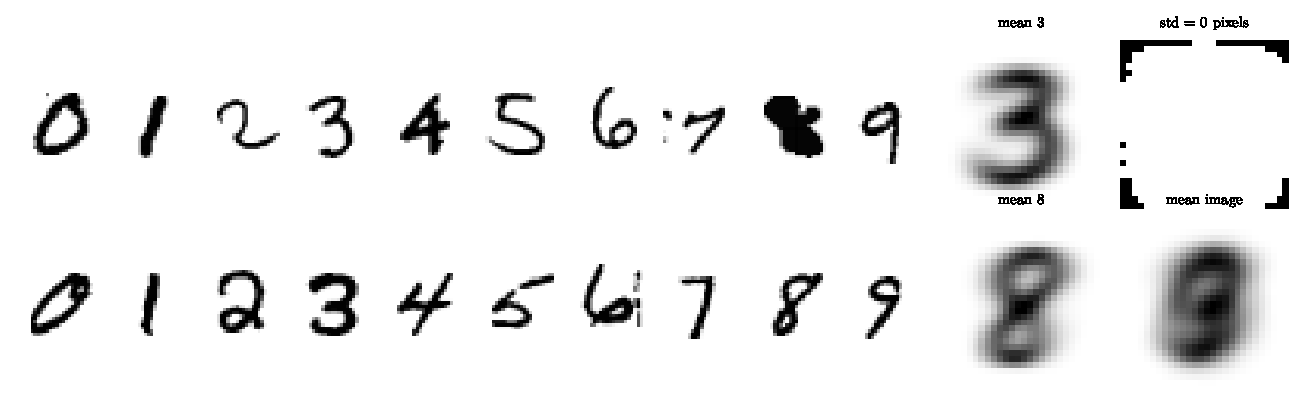
\includegraphics[width=0.95\textwidth]{../results/figures/eda_overview.pdf}
\caption{Khảo sát dữ liệu huấn luyện. Hai hàng đầu: mẫu ngẫu nhiên của mỗi chữ số. Bên phải: ảnh trung bình của lớp 3 và lớp 8, bản đồ các pixel có phương sai bằng 0 (màu đen), và ảnh trung bình toàn tập.}
\label{fig:eda}
\end{figure}

\textbf{Khảo sát.} Các lớp gần cân bằng: lớp 1 chiếm nhiều nhất ($11.24\%$) và lớp 5 ít nhất ($9.03\%$), nên accuracy là chỉ số hợp lý; macro precision, recall và F1 vẫn được báo cáo để lớp ít mẫu không bị che khuất. Khoảng $81\%$ giá trị điểm ảnh là nền, và $71$ vị trí ở viền ảnh luôn bằng nền trên tập train (\cref{fig:eda}); chúng làm phương sai ước lượng của Naïve Bayes bằng 0 và không bao giờ được cây quyết định chọn để tách. Hệ số tương quan Pearson giữa hai pixel kề nhau theo chiều ngang, tính trong từng lớp rồi lấy trung bình trên các vị trí có phương sai khác 0, là $\corrAdj$; giả thiết độc lập có điều kiện của Naïve Bayes (mục~\ref{sec:nb}) vì vậy không thỏa mãn trên dữ liệu này.

\textbf{Khác biệt phân phối.} Validation là một phần của tập huấn luyện chính thức, còn test chính thức là tập tách riêng. Cả năm mô hình đều có độ chính xác test không thấp hơn validation (\cref{tab:accuracy}); chênh lệch là $1.65$ điểm với Naïve Bayes, $0.37$ điểm với softmax và không quá $0.15$ điểm với ba mô hình còn lại. Chúng tôi không khảo sát nguyên nhân và chỉ dùng validation để chọn mô hình.
